\chapter[Cortical magnetization transfer abnormalities and connectome dysconnectivity in schizophrenia]{Cortical magnetization transfer abnormalities and connectome dysconnectivity \\in schizophrenia}

\chaptermark{MTR abnormalities and dysconnectivity in schizophrenia}

\label{ch:mtrscz}

\begin{flushright}
\textit{Yongbin Wei, Guusje Collin, René C.W. Mandl, Wiepke Cahn, Kristin Keunen, \\Ruben Schmidt, René S. Kahn, Martijn P. van den Heuvel,
}\\
Schizophrenia Research, 2018; 192: 172-178
\vspace{7 mm}

\end{flushright}

\begin{refsection}
\newpage
\section*{Abstract}
Macroscale dysconnectivity in schizophrenia is associated with neuropathological abnormalities. The extent to which alterations in cortical myelination as revealed in vivo by magnetization transfer ratio (MTR) are related to macroscale dysconnectivity remains unknown. We acquired magnetization transfer imaging (MTI) data and diffusion weighted imaging (DWI) data from 78 schizophrenia patients and 93 healthy controls for MTR extraction and connectome reconstruction to examine the possible link between cortical myelination and macroscale dysconnectivity. Our findings showed significant cortical MTR disruptions in several prefrontal areas in schizophrenia patients, including bilateral rostral middle frontal areas, right pars orbitalis, and right frontal pole. Furthermore, cortical MTR alterations between patients and controls were significantly correlated with the level of regional disconnectivity. Together, our findings provide evidence that microstructural neuropathological abnormalities in schizophrenia are predominately present in prefrontal areas of the cortex and are associated with alterations in structural connectome architecture at the whole brain network level.

\section*{Introduction}
Schizophrenia is a severe psychiatric disorder that is characterized as a disorder of brain connectivity \citep{Fornito2012SchizophreniaNA,Stephan2009DysconnectionIS,Heuvel2014BrainNI}. In the past two decades, empirical magnetic resonance imaging (MRI) studies have provided a large body of evidence for disruptions of interregional connectivity \citep{EllisonWright2009MetaanalysisOD,Fornito2012SchizophreniaNA,Klauser2017WhiteMD,Fitzsimmons2013ReviewOF}. Connectome studies focused on brain network topology offer further support for this hypothesis by presenting converging evidence of decreased network efficiency \citep{Zalesky2011DisruptedAF}, less centralized frontal and parietal hubs \citep{vanDenHeuvel2010AberrantFA}, and reduced rich club organization in schizophrenia \citep{Collin2014ImpairedRC,vanDenHeuvel2013AbnormalRC}.

In terms of microscale neuropathology in schizophrenia, a wide range of histological alterations have been observed in the cerebral cortex (for a review, see \citep{Bakhshi2015TheNO}). Findings include increased neuronal density \citep{DorphPetersen2009PyramidalNN,Selemon1995AbnormallyHN,Selemon1998ElevatedND,Yang2011IncreasedIW}, decreased neuron size \citep{Chana2003TwodimensionalAO,Rajkowska1998NeuronalAG}, reduced dendritic spines density \citep{Garey1998ReducedDS,Glantz2000DecreasedDS,Glausier2013DendriticSP,Penzes2011DendriticSP} and reduced oligodendroglia density \citep{Uranova2004OligodendroglialDI,Uranova2001ElectronMO,Vostrikov2013ReducedOD}. Alterations in neuronal, synaptic and dendritic density have been suggested to underlie gray matter changes as revealed by neuroimaging studies \citep{Fornito2009AnatomicalAO,Fornito2009ReconcilingNA} and oligodendrocyte and myelination dysfunction have been linked to perturbations of white matter connectivity in schizophrenia \citep{Cassoli2015DisturbedMI}. In a recent study, we confirmed the pattern of abnormalities in spine density of pyramidal neurons across the cortex to be associated with the pattern of white matter connectivity changes in schizophrenia \citep{VANDENHEUVEL2016293}.

Magnetization transfer ratio (MTR) obtained by means of magnetization transfer imaging (MTI) provides an estimate of in vivo brain microstructure, in particular myelination levels \citep{Whitaker2016AdolescenceIA}, a technique that could complement post-mortem investigations of neuronal structure. MTR detects subtle changes in protons that are tightly bound to macromolecular structures, such as myelin, cell membrane proteins, and phospholipids \citep{wolff1994magnetization}. Indeed, MTR reductions in white matter have been shown to be associated with myelin loss in demyelinating diseases such as multiple sclerosis \citep{Chen2007VoxelbasedAO,Chen2008MagnetizationTR,Derakhshan2014SurfacebasedAR,Dousset1992ExperimentalAE,Schmierer2004MagnetizationTR,schmierer2007quantitative}, making MTR a suitable metric for demyelination in neurological conditions. In schizophrenia, several studies have revealed MTR changes in temporal \citep{Foong2000InVI} and occipital white matter \citep{Palaniyappan2013CombinedWM}, the occipito-frontal fasciculus \citep{Kubicki2005DTIAM}, and the right uncinate fasciculus \citep{Mandl2010TractbasedAO}.

MTR has also been used to assess the microstructure of gray matter. MTR studies have verified region-specific cortical myelination patterns in the healthy human brain \citep{Whitaker2016AdolescenceIA} with high myelin levels in primary cortices \citep{Glasser2014TrendsAP,Shafee2015GrayMM} and MTI-derived myelination estimates have been observed to be associated with oligodendroglia-related genes in the healthy human brain \citep{Whitaker2016AdolescenceIA}. Studies in schizophrenia have reported MTR changes in frontal and temporal regions \citep{Bagary2003GrayAW,Foong2001NeuropathologicalAI,Price2010BrainPI}, insula \citep{Bagary2003GrayAW}, and the cingulate gyri \citep{Price2010BrainPI}. It remains unknown whether such neuropathological alterations as revealed by intracortical MTR changes are associated with disruptions in macroscale white matter connectivity.

In the current study, we use MTR measurements to characterize neuropathological abnormalities in schizophrenia. Based on the afore-mentioned findings of cortical microscale alterations associated with macroscale connectivity changes in schizophrenia \citep{VANDENHEUVEL2016293}, we hypothesize that cortical MTR abnormalities may relate to macroscale dysconnectivity in the structural connectome. To test this hypothesis, we use a set of MTI data, diffusion weighted imaging (DWI) data and T1-weighted imaging data in 78 schizophrenia patients and 93 healthy controls for MTR extraction and structural connectome reconstruction. We demonstrate cortical MTR differences between schizophrenia patients and healthy controls and show that these cortical MTR alterations correlate with global white matter connectivity disruptions.

\section*{Methods}
\subsection*{Subjects}
A total of 171 subjects participated in this study, including 78 schizophrenia patients and 93 healthy controls. Subjects were included as part of the Genetic Risk and Outcome of Psychosis (GROUP) cohort study at the University Medical Center Utrecht, the Netherlands. The affiliated medical ethics committee approved the study and written informed consent was obtained from each subject before study participation. Two patients and four controls were excluded because no MTI or DWI data was acquired. Detailed demographics of the remaining subjects (i.e., 76 patients and 89 controls) are listed in Table \ref{mtrtable1}. A higher proportion of males were included in the patient group (42 males and 47 females in controls, 62 males and 14 females in schizophrenia patients). All subjects went through an extensive psychiatric assessment procedure to determine the presence or absence of psychopathology, by using the Comprehensive Assessment of Symptoms and History (CASH) \citep{Andreasen1992TheCA}. Patients met Diagnostic and Statistical Manuals for Mental Disorders Fourth Edition (DSM-IV) \citep{american2013diagnostic} criteria for schizophrenia or related spectrum disorders. Control subjects were eligible for inclusion if they had no current or lifetime psychiatric disorder and no first- or second-degree relatives with a psychotic disorder.

At the time of scanning, 60 out of 76 patients were taking typical or atypical antipsychotic medication. The type and daily dose of antipsychotic medication were recorded and converted to a haloperidol equivalent dose using conversion rates \citep{Kroken2009TreatmentOS}. The severity of symptoms was estimated using the Positive And Negative Syndrome Scale (PANSS) \citep{Kay1987ThePA}. The presence and severity of subclinical symptoms in controls were assessed using the Community Assessment of Psychic Experiences (CAPE) \citep{Stefanis2002EvidenceTT}. For all subjects, total IQ was assessed using four subtests of the Dutch version of Wechsler Adult Intelligence Scale (WAIS), including Vocabulary, Comprehension, Block Design and Picture Arrangement \citep{WAIS}. The Word Learning Task (WLT) was performed to assess verbal learning and memory abilities \citep{Brand1985LearningAR}. Statistical analyses on group differences in demographic and clinical characteristics were performed by using two-sample t-test for continuous variables and chi-squared tests for categorical variables (Table \ref{mtrtable1}).

\begin{sidewaystable}
\renewcommand{\arraystretch}{0.8}
\centering
\small
\fontfamily{phv}\selectfont
\captionof{table}{Demographic and clinical characteristics.}
\begin{tabular}{@{}llll@{}}
\toprule
                                                        & Controls (\textit{N} = 89)          & Patients (\textit{N} = 76)          & \textit{P}                 \\ \midrule
Age in years, mean (SD), {[}range{]}                    & 26.6 (7.7) {[}17–49{]}     & 26.3 (5.4) {[}16–43{]}     & 0.79\textsuperscript{a}             \\
Gender, M/F                                             & 42/47                      & 62/14                      & \textless 0.0001\textsuperscript{b} \\
DSM-diagnosis                                           &                            &                            &                   \\
Schizophrenia, N (\%)                                   & -                          & 51 (67.1)                  & -                 \\
Schizophreniform disorder, N (\%)                       & -                          & 3 (4.0)                    & -                 \\
Schizoaffective disorder, N (\%)                        & -                          & 10 (13.2)                  & -                 \\
Other\textsuperscript{c}, N (\%)                                          & -                          & 9 (11.8)                   & -                 \\
Bipolar disorder, N (\%)                                & -                          & 3 (4.0)                    & -                 \\
IQ, mean (SD) {[}range{]}                               & 114.6 (15.2) {[}83–144{]}  & 93.2 (13.5) {[}63–128{]}   & \textless 0.0001\textsuperscript{a} \\
PANSS symptoms                                          &                            &                            &                   \\
Total, mean (SD) {[}range{]}                            & -                          & 61.6 (18.1) {[}32–107{]}   & -                 \\
Positive, mean (SD) {[}range{]}                         & -                          & 15.2 (5.5) {[}7–29{]}      & -                 \\
Negative, mean (SD) {[}range{]}                         & -                          & 15.5 (6.1) {[}7–31{]}      & -                 \\
General, mean (SD) {[}range{]}                          & -                          & 30.9 (8.9) {[}17–59{]}     & -                 \\
CAPE subclinical symptoms                               &                            &                            &                   \\
Total, mean (SD) {[}range{]}                            & 0.34 (0.22) {[}0–1.05{]}   & -                          & -                 \\
Positive, mean (SD) {[}range{]}                         & 0.19 (0.21) {[}0–1.00{]}   & -                          & -                 \\
Negative, mean (SD) {[}range{]}                         & 0.46 (0.32) {[}0–1.50{]}   & -                          & -                 \\
General, mean (SD) {[}range{]}                          & 0.52 (0.30) {[}0–1.63{]}   & -                          & -                 \\
Antipsychotic medication                                &                            &                            &                   \\
Typical/atypical/none/unknown, N\textsuperscript{d}                       & -                          & 4/56/10/6                  & -                 \\
Haloperidol equivalent dose (mg), mean (SD) {[}range{]} & -                          & 9.4 (6.4) {[}0.75–32{]}    & -                 \\
WLT\textsuperscript{e}                                                    &                            &                            &                   \\
Delayed recall correct items, mean (SD) {[}range{]}     & 21.10 (13.80) {[}0–36{]}   & 19.83 (8.11) {[}0–36{]}    & 0.50\textsuperscript{a}             \\
Immediate recall correct items, mean (SD) {[}range{]}   & 7.01 (4.97) {[}0–15{]}     & 6.16 (3.25) {[}0–14{]}     & 0.22\textsuperscript{a}             \\
Retention rate, mean (SD) {[}range{]}                   & 0.81 (0.17) {[}0.2–1.17{]} & 0.74 (0.23) {[}0.09–1.4{]} & 0.07\textsuperscript{a}             \\ \bottomrule
\end{tabular}
\begin{flushleft}
\footnotesize
Note: DSM, Diagnostic and Statistical Manuals; PANSS, Positive And Negative Syndrome Scale; CAPE, Community Assessment of Psychic Experiences; WLT, Word Learning Task. \textsuperscript{a} Two sample t-test. \textsuperscript{b} Chi-square test, statistically different between two groups.
\textsuperscript{c} Other diagnoses include brief psychotic disorder, psychotic disorder not otherwise specified, and delusional disorder. \textsuperscript{d} “Typical”: haloperidol, perfluridol and perfenazine; “atypical”: risperidone, olanzapine, quetiapine, clozapine, aripiprazole; “none”: no current antipsychotic treatment. \textsuperscript{e} Data were missing 10 schizophrenia patients and 25 controls.
\end{flushleft}
\label{mtrtable1}
\end{sidewaystable}

\subsection*{Data acquisition}
For each subject, a T1-weighted scan, an MTI scan and a DWI scan were acquired on a 1.5 Tesla Intera Achieva Philips System at the University Medical Center Utrecht using a 6-element SENSE receiver head coil. First, the 3-dimensional T1-weighted coronal (spoiled gradient) echo scan was acquired with following scanning parameters: acquisition matrix = 256 $\times$ 256; echo time (TE) = 4.6 ms; repetition time (TR) = 30 ms; flip angle = 30$^{\circ}$; 160-180 contiguous slices; scan duration = 405-456 s; voxel size = 1 $\times$ 1 $\times$ 1.2 mm\textsuperscript{3}; field of view (FOV) = 256 $\times$ mm\textsuperscript{2}; SENSE factor = 1.5/1.5. Second, an MTR scan was acquired using 3-dimensional magnetization transfer imaging comprising 2 volumes (transverse; acquisition matrix = 128 $\times$ 128; TE = 3.7 ms; TR = 37.5 ms; flip angle = 8$^{\circ}$; 60 slices of 2.5 mm; FOV = 240 $\times$ 240 mm\textsuperscript{2}; SENSE factor = 2.5, scan duration = 394 s). For the second volume, an additional off-resonance prepulse was applied (frequency offset = 1100 Hz; 620$^{\circ}$; three-lobe sync-shaped). Third, two sets of DWI scans were acquired to reconstruct the white matter pathways (8 unweighted volumes with b = 0 s/mm\textsuperscript{2} and 32 non-collinear diffusion-unweighted volumes with b-factor = 1000 s/mm\textsuperscript{2}; acquisition matrix = 96 $\times$ 96; reconstruction matrix = 128 $\times$ 128; FOV = 240 $\times$ 240 mm\textsuperscript{2}; TE = 88 ms; TR = 9822 ms; flip angle = 90$^{\circ}$; 60 slices of 2.5 mm; no slice gap; SENSE factor = 2.5; scan duration = 296 s).

\subsection*{Data preprocessing}
\subsubsection*{T1-weighted data}
Three-dimensional T1-weighted data was acquired for white and gray matter tissue segmentation and cortical mantle reconstruction, which were performed with the FreeSurfer software package \citep{FISCHL2012Freesurfer}. The reconstructed cortical mantle was parcellated into 114 distinct cortical regions (i.e., 57 regions per hemisphere) according to a subdivision of the Desikan-Killiany atlas \citep{Fischl2004parcellation,CAMMOUN2012386,DESIKAN2006968}.

\subsubsection*{MTI data}
MTI data of two volumes, including the first volume without the magnetization prepulse (\textit{I\textsubscript{0}}) and the second volume with the magnetization prepulse (\textit{I\textsubscript{m}}), were utilized to compute cortical MTR values. The \textit{I\textsubscript{m}} volume was rigidly aligned with the \textit{I\textsubscript{0}} volume taking the mutual information as a similarity metric. MTR maps were obtained by calculating the ratio of reduction between \textit{I\textsubscript{0}} and \textit{I\textsubscript{m}} according to the equation MTR = (\textit{I\textsubscript{0}} - \textit{I\textsubscript{m}}) / \textit{I\textsubscript{0}} × 100\%. The ratio varies between 0 and 100\% reflecting no (i.e., \textit{I\textsubscript{0}} = \textit{I\textsubscript{m}}) to complete (i.e., \textit{I\textsubscript{0}} $\mathsf{\gg}$ \textit{I\textsubscript{m}}) signal reduction caused by magnetization transfer.

MTR and cortical parcellation maps were rigidly aligned with the un-weighted B0 image of the DWI data using mutual information as a similarity metric. The mean MTR within each cortical region was calculated for each subject, taking the partial volume effect into account:\\
\[ \mathsf{MTR_{i} = \frac{\sum_{n\in i} P_{GM,n} \times MTR_{n}}{\sum_{n\in i} P_{GM,n}} } \]\\
where \textit{n} is the voxel index within the region \textit{i} and \textit{P}\textsubscript{GM,n} is the percentage of gray matter volume for the voxel \textit{n}. \textit{P}\textsubscript{GM,n} was calculated by selecting all corresponding voxels in the T1-weighted images for the voxel \textit{n} in MTR images and computing the proportion of the voxels classified as gray matter. \textit{P}\textsubscript{GM} ranged from 0\% to 100\% indicating a non-gray-matter voxel or a voxel filled completely with gray matter, respectively. Regions of bilateral inferiortemporal\_1, inferiortemporal\_2, and medialorbitofrontal\_1, and right mediaorbitofrontal\_2 were excluded from following analyses due to signal artifacts in the raw images across subjects, leaving mean MTR values for 107 remaining cortical regions per subject. The reliability of MTR signals was examined in three ways, including analyses of tissue contrast, signal noise ratio (SNR), and individual variance (see Supplementary Information).

\subsubsection*{DWI data}
DWI scans were acquired for the reconstruction of white matter pathways. First, two sets of b = 0 volumes were averaged and the 2 $\times$ 32 diffusion directions were realigned and corrected for small head movements and common gradient-induced distortions \citep{ANDERSSON2002177}. Second, a diffusion profile was reconstructed for each voxel within the brain mask using a combination of compressed sensing techniques (CFARI) \citep{Landman2012ResolutionOC} and robust tensor fitting approaches, which allow reconstruction of complex fiber achitectures and maintain high accuracy in voxels with one dominant diffusion direction. A tensor was used to describe the diffusion profile unless compressed sensing indicated the existence of multiple pronounced diffusion directions. Third, the white matter pathways were reconstructed using deterministic streamline tractography (suited for multi-direction approaches). For each voxel within the brain mask, eight streamline seeds were started and tracking was stopped if the streamline reached a voxel of low preferred diffusion direction (fractional anisotropy < 0.1), exceeded the gray matter/white matter mask, or made a sharp turn (>45 degrees).

\subsection*{Connectome analysis}
A brain structural network was constructed from the collection of reconstructed tractography streamlines and the individual parcellation map containing 114 cortical regions derived from subdivisions of the Desikan-Killiany atlas \citep{CAMMOUN2012386,DESIKAN2006968,Fischl2004parcellation}. Each network was illustrated by a graph G = (V, E), where V indicates a set of nodes (i.e., all cortical regions) and E indicates a set of edges between the nodes (i.e., the total collection of reconstructed white matter streamlines). Network nodes were defined as connected when a set of reconstructed streamlines interconnected them. If no streamline was found, nodes were regarded as unconnected. The absolute number of reconstructed streamlines (NOS) was taken as the connection weight. In addition, connections were also weighted by the streamline density (dividing NOS by the mean volume of two connected regions). Streamline density corrected the potential effect of regional volume on NOS \citep{Hagmann2008MappingTS,vanDenHeuvel2011RichclubOO}. The connectivity strength of each cortical region was acquired by computing the total sum of weights (i.e., NOS or streamline density) of their connections.

\subsection*{Statistical analysis}
\subsubsection*{Between-group MTR analysis}
The non-parametric Wilcoxon Rank Sum permutation analysis was used to examine MTR differences between schizophrenia patients and healthy controls. Cortical thickness, gray matter volume and age were first regressed out from MTR using a general linear model. A Wilcoxon Rank Sum test was performed using MTR residuals from the two groups, resulting in a ranksum value indicating the extent to which the medians of the two groups differed. Next, 10,000 permutations of group assignment were performed to randomly assign subjects to two groups with the same size as the original groups. For each of 10,000 repetitions, the ranksum value was recomputed using the Wilcoxon Rank Sum test to generate an empirical null-distribution. The original ranksum value was then compared to the null-distribution.  A two-tailed p-value was assigned according to the proportion of random permutations that exceeded the original ranksum value. To control for multiple comparisons, false discovery rate (FDR) correction was performed. Results were considered statistically significant if \textit{q} < 0.05. Due to the uneven distribution of gender across the groups in our sample, MTR group differences were reassessed by two ways: using male and female subjects only and adopting a subgroup of gender-matched controls (see Supplementary Information).

\subsubsection*{Correlation analysis between MTR and clinical variables}
We correlated MTR measurements with clinical characteristics using Pearson’s correlation for regions showing significant between-group MTR differences. Clinical variables included PANSS, estimated total IQ, WAIS subtest (e.g., Vocabulary, Comprehension, Block Design and Picture Arrangement) scores, and WLT variables (e.g., Delayed recall correct items, Immediate recall correct items and Retention rate). Effects reaching \textit{q} < 0.05 (FDR corrected) were considered statistically significant.

\subsubsection*{Correlation analysis between alterations in MTR and connectivity}
The level of MTR change for each region was represented as the ratio of change between patients and controls (i.e., {[}Patients - Controls{]} / {[}Controls{]}). Likewise, the level of connectivity change for each region was assessed as the ratio of between-group changes in connectivity strength. Across all cortical regions, Pearson’s correlations were computed between the pattern of change in MTR and the cortical pattern of change in connectivity. Partial correlations were also calculated between the cortical pattern of changes of MTR and connectivity. Between-group differences in cortical thickness and volume (computed as the percentage of change in group-averaged thickness and volume) were included as covariates. Ranksum values resulting from between-group Wilcoxon Rank Sum test of MTR or connectivity strength were taken as an alternative measurement of between-group differences.


\section*{Results}
\subsection*{MTR differences between schizophrenia patients and controls}
A significant reduction in cortical MTR was found for the bilateral rostral middle frontal area (left: \pval = 0.0002 and right: \pval = 0.0004), the right pars orbitalis (\pval = 0.0012), and the right frontal pole (\pval = 0.0006) in schizophrenia patients as compared to healthy controls (\textit{q} < 0.05, FDR correction) (Figure \ref{mtrFig1}). Additional analyses on the gender effect showed that these prefrontal MTR reductions might be not driven by group differences in gender distribution (see Supplementary Information).

\begin{figure}[h]
    \centering
    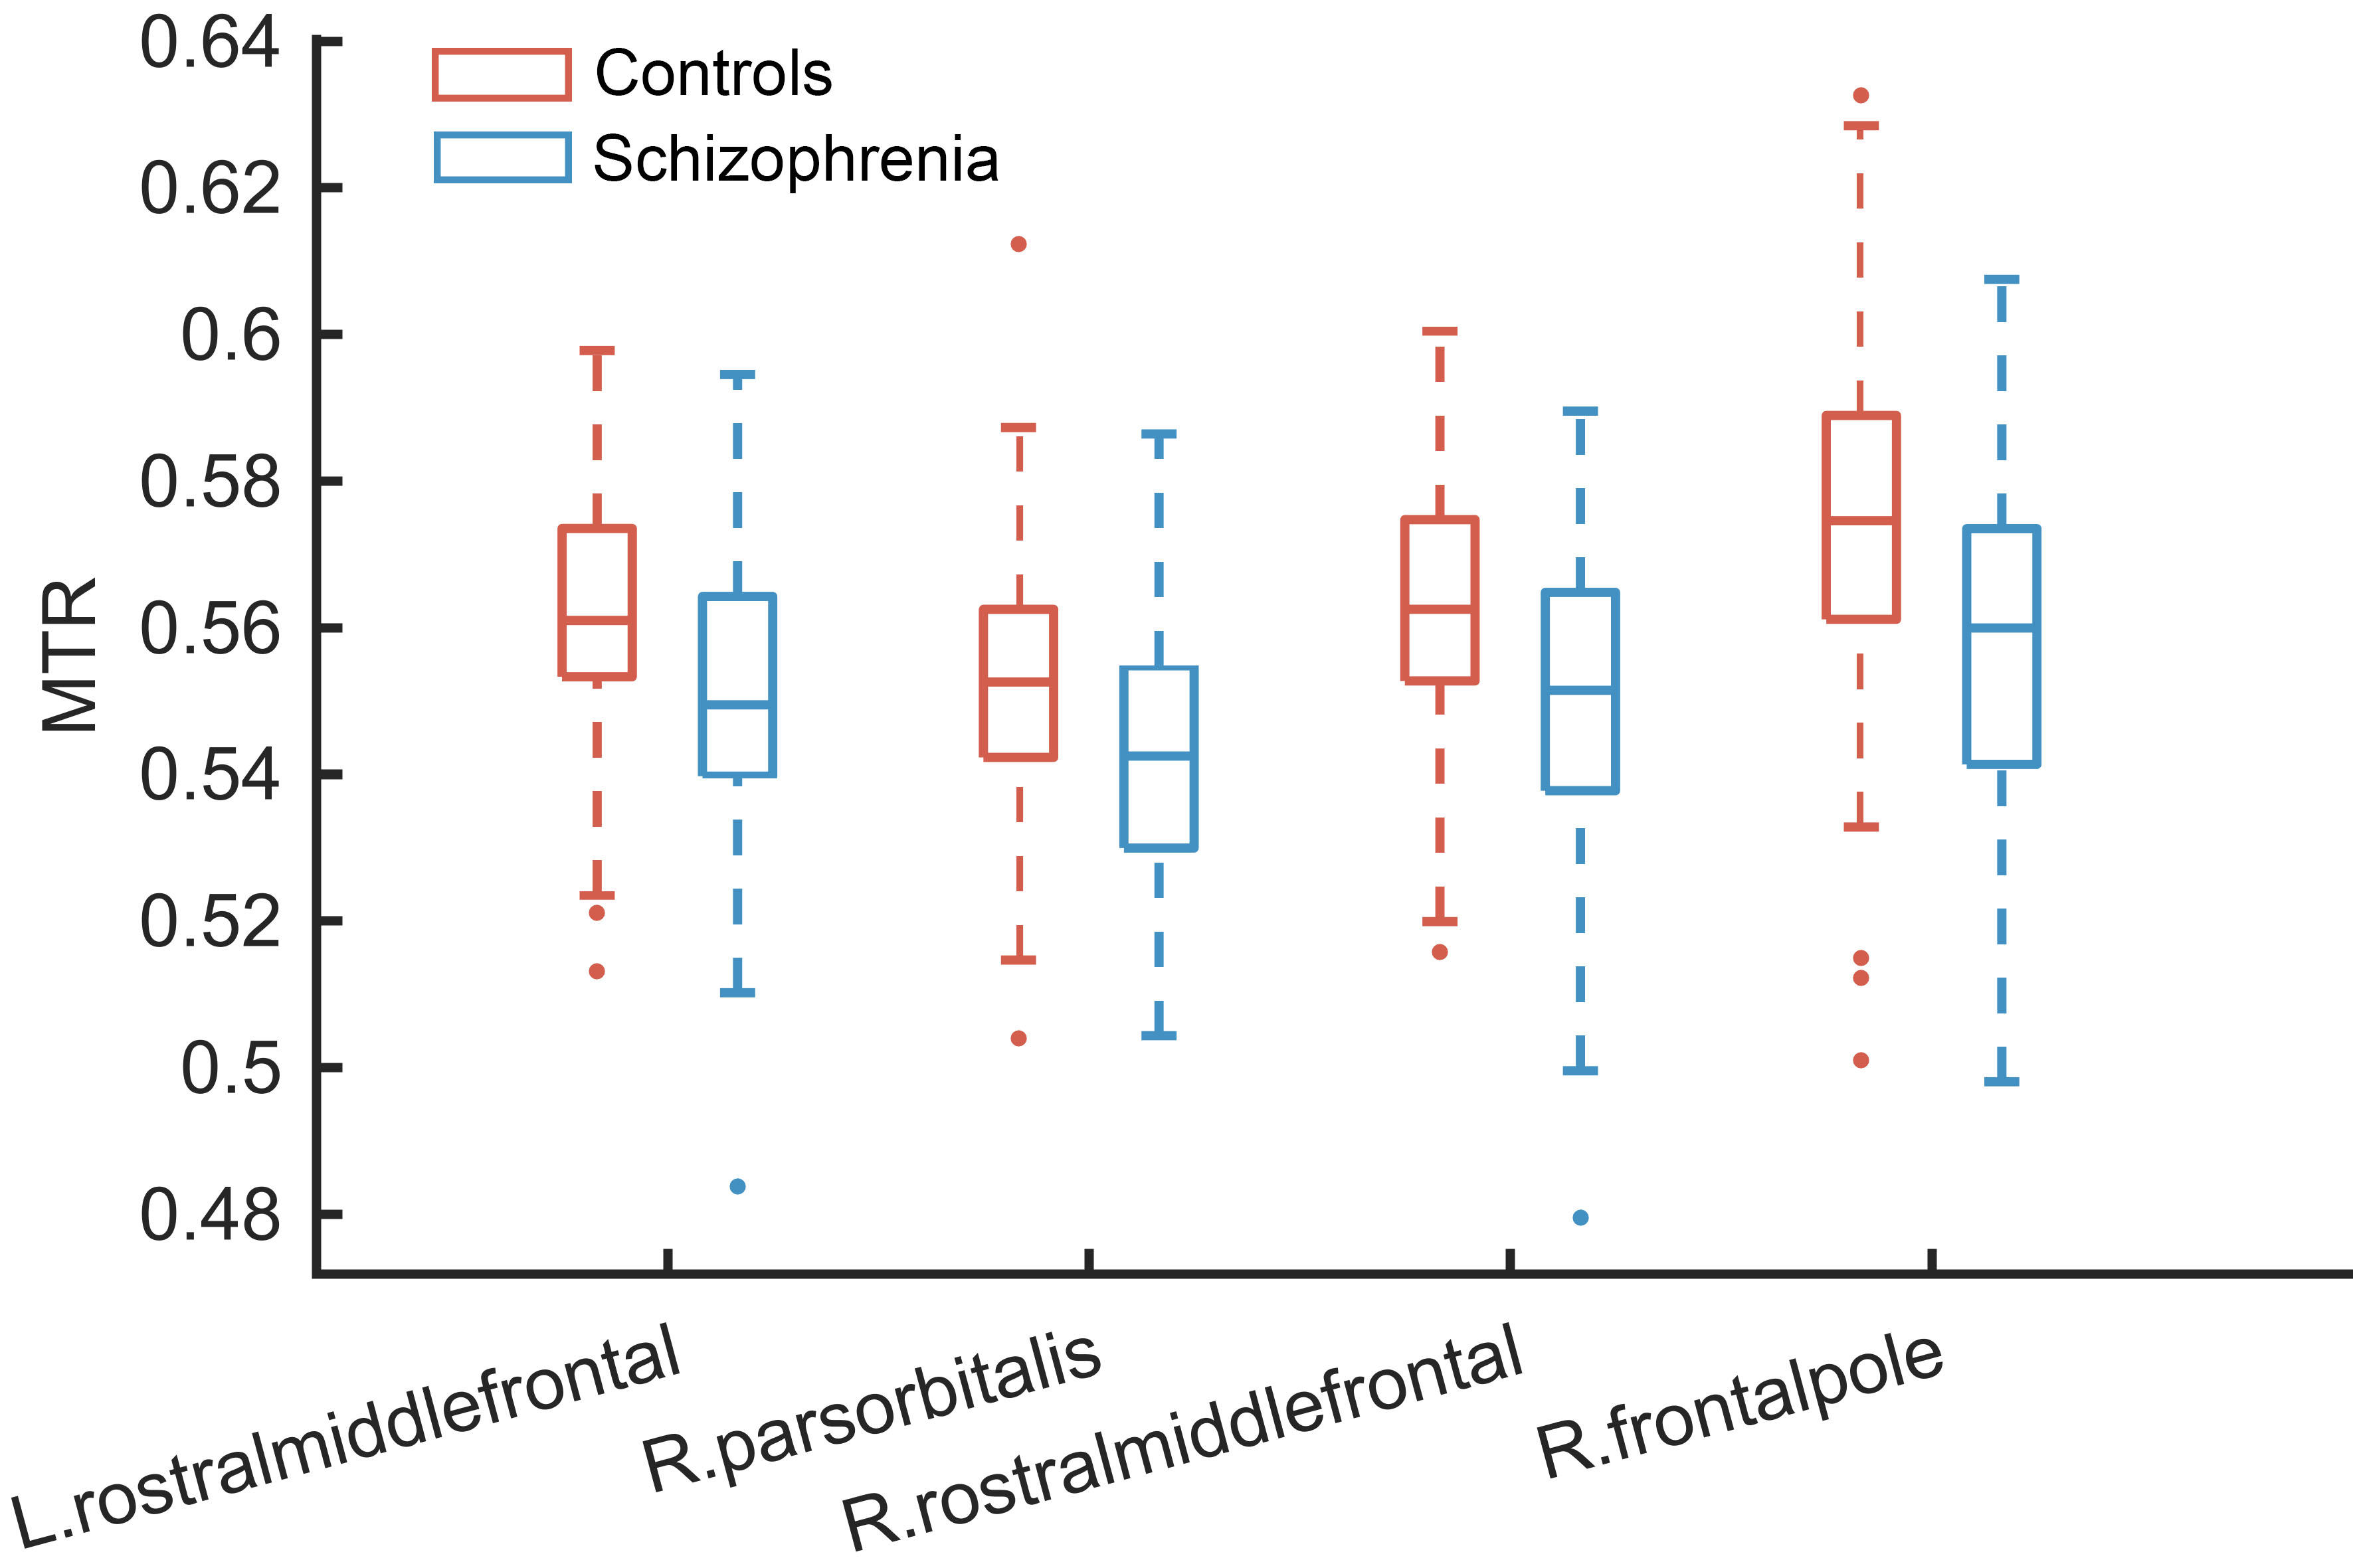
\includegraphics[width=8cm]{images/mtrFig1.jpg}
    \caption{Boxplots of MTR in the bilateral rostral middle frontal area, right pars orbitalis and right frontal pole. The central mark on each box is the median, the edges of the box are the 25th and 75th percentiles, the whiskers extend to the most extreme data points considered not to be outliers according to interquartile range (IQR) algorithm, with outliers plotted individually. Red: controls, blue: schizophrenia patients. L: left hemisphere, R: right hemisphere.}
    \label{mtrFig1}
\end{figure}

\begin{figure}[H]
    \centering
    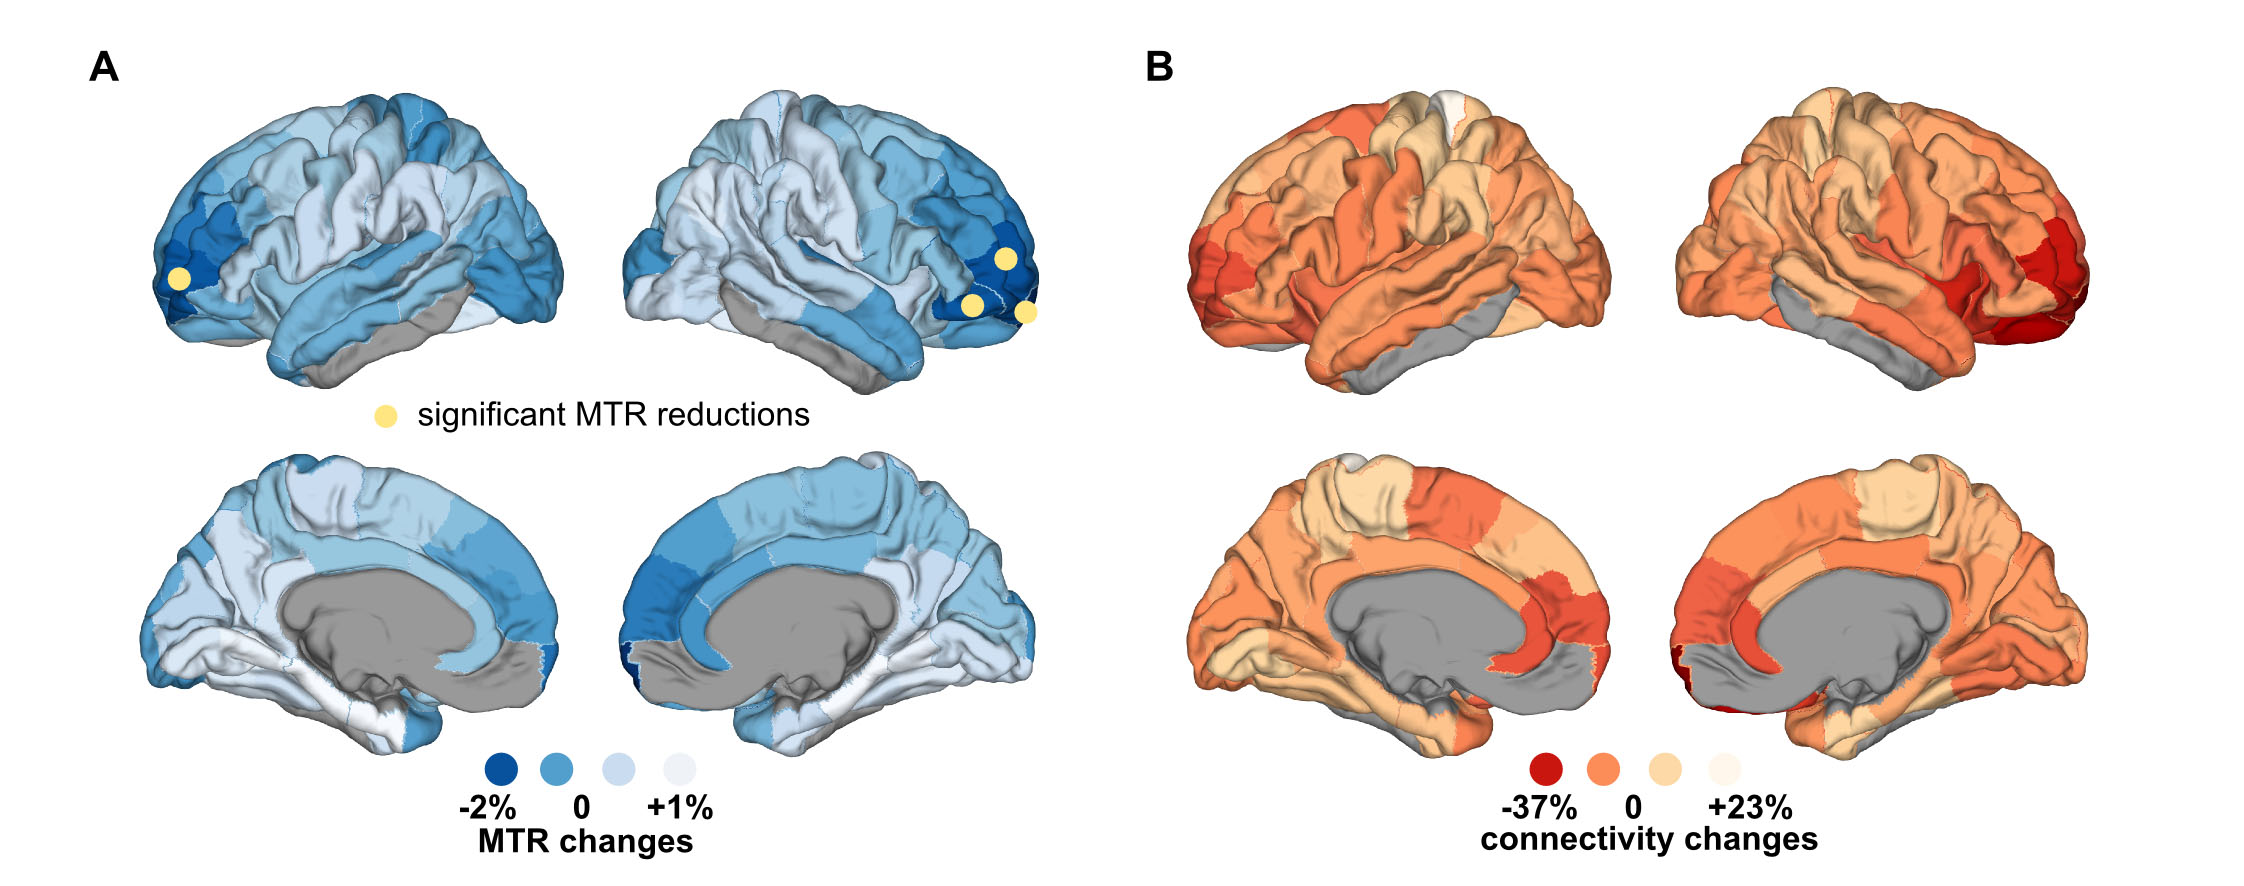
\includegraphics[width=\linewidth]{images/mtrFig2.jpg}
    \caption{Surface maps of between-group changes in MTR and connectivity strength (NOS). (A) Changes for group-averaged MTR between schizophrenia patients and controls (i.e., {[}Patient – Control{]}/Control) are illustrated. Yellow dots indicate cortical regions showing significant MTR differences between the two groups; (B) Changes for group-averaged connectivity strength (NOS) between schizophrenia patients and controls are presented.}
    \label{mtrFig2}
\end{figure}

\subsection*{Associations between MTR and clinical variables}
Cortical MTR of the regions showing significant MTR differences between schizophrenia patients and controls were tested for associations with clinical symptoms and IQ in patients. There were no significant correlations with positive, negative, total and general PANSS symptoms, nor with IQ and WAIS subtest scores. Only weak correlations were found between the WLT retention rate and cortical MTR in right rostral middle frontal area (\rval = 0.26, \pval = 0.0355, not corrected) and right frontal pole (\rval = 0.28, \pval = 0.0224, not corrected) in schizophrenia patients.

\subsection*{Associations between MTR alterations and disconnectivity}
Cortical maps of MTR alterations and connectivity strength (NOS) changes between schizophrenia patients and controls are illustrated in Figure \ref{mtrFig2}. Regional reductions in MTR were significantly associated with differences in connectivity strength (NOS, \rval = 0.40, \pval < 0.0001) (Figure \ref{mtrFig3}), suggesting that regions with the largest regional MTR reductions also show the largest reductions in macroscale connectivity strength. Examining streamline density yielded similar results (\rval = 0.40, \pval < 0.0001) (Figure \ref{mtrFig4}).

\begin{figure}[h]
    \centering
    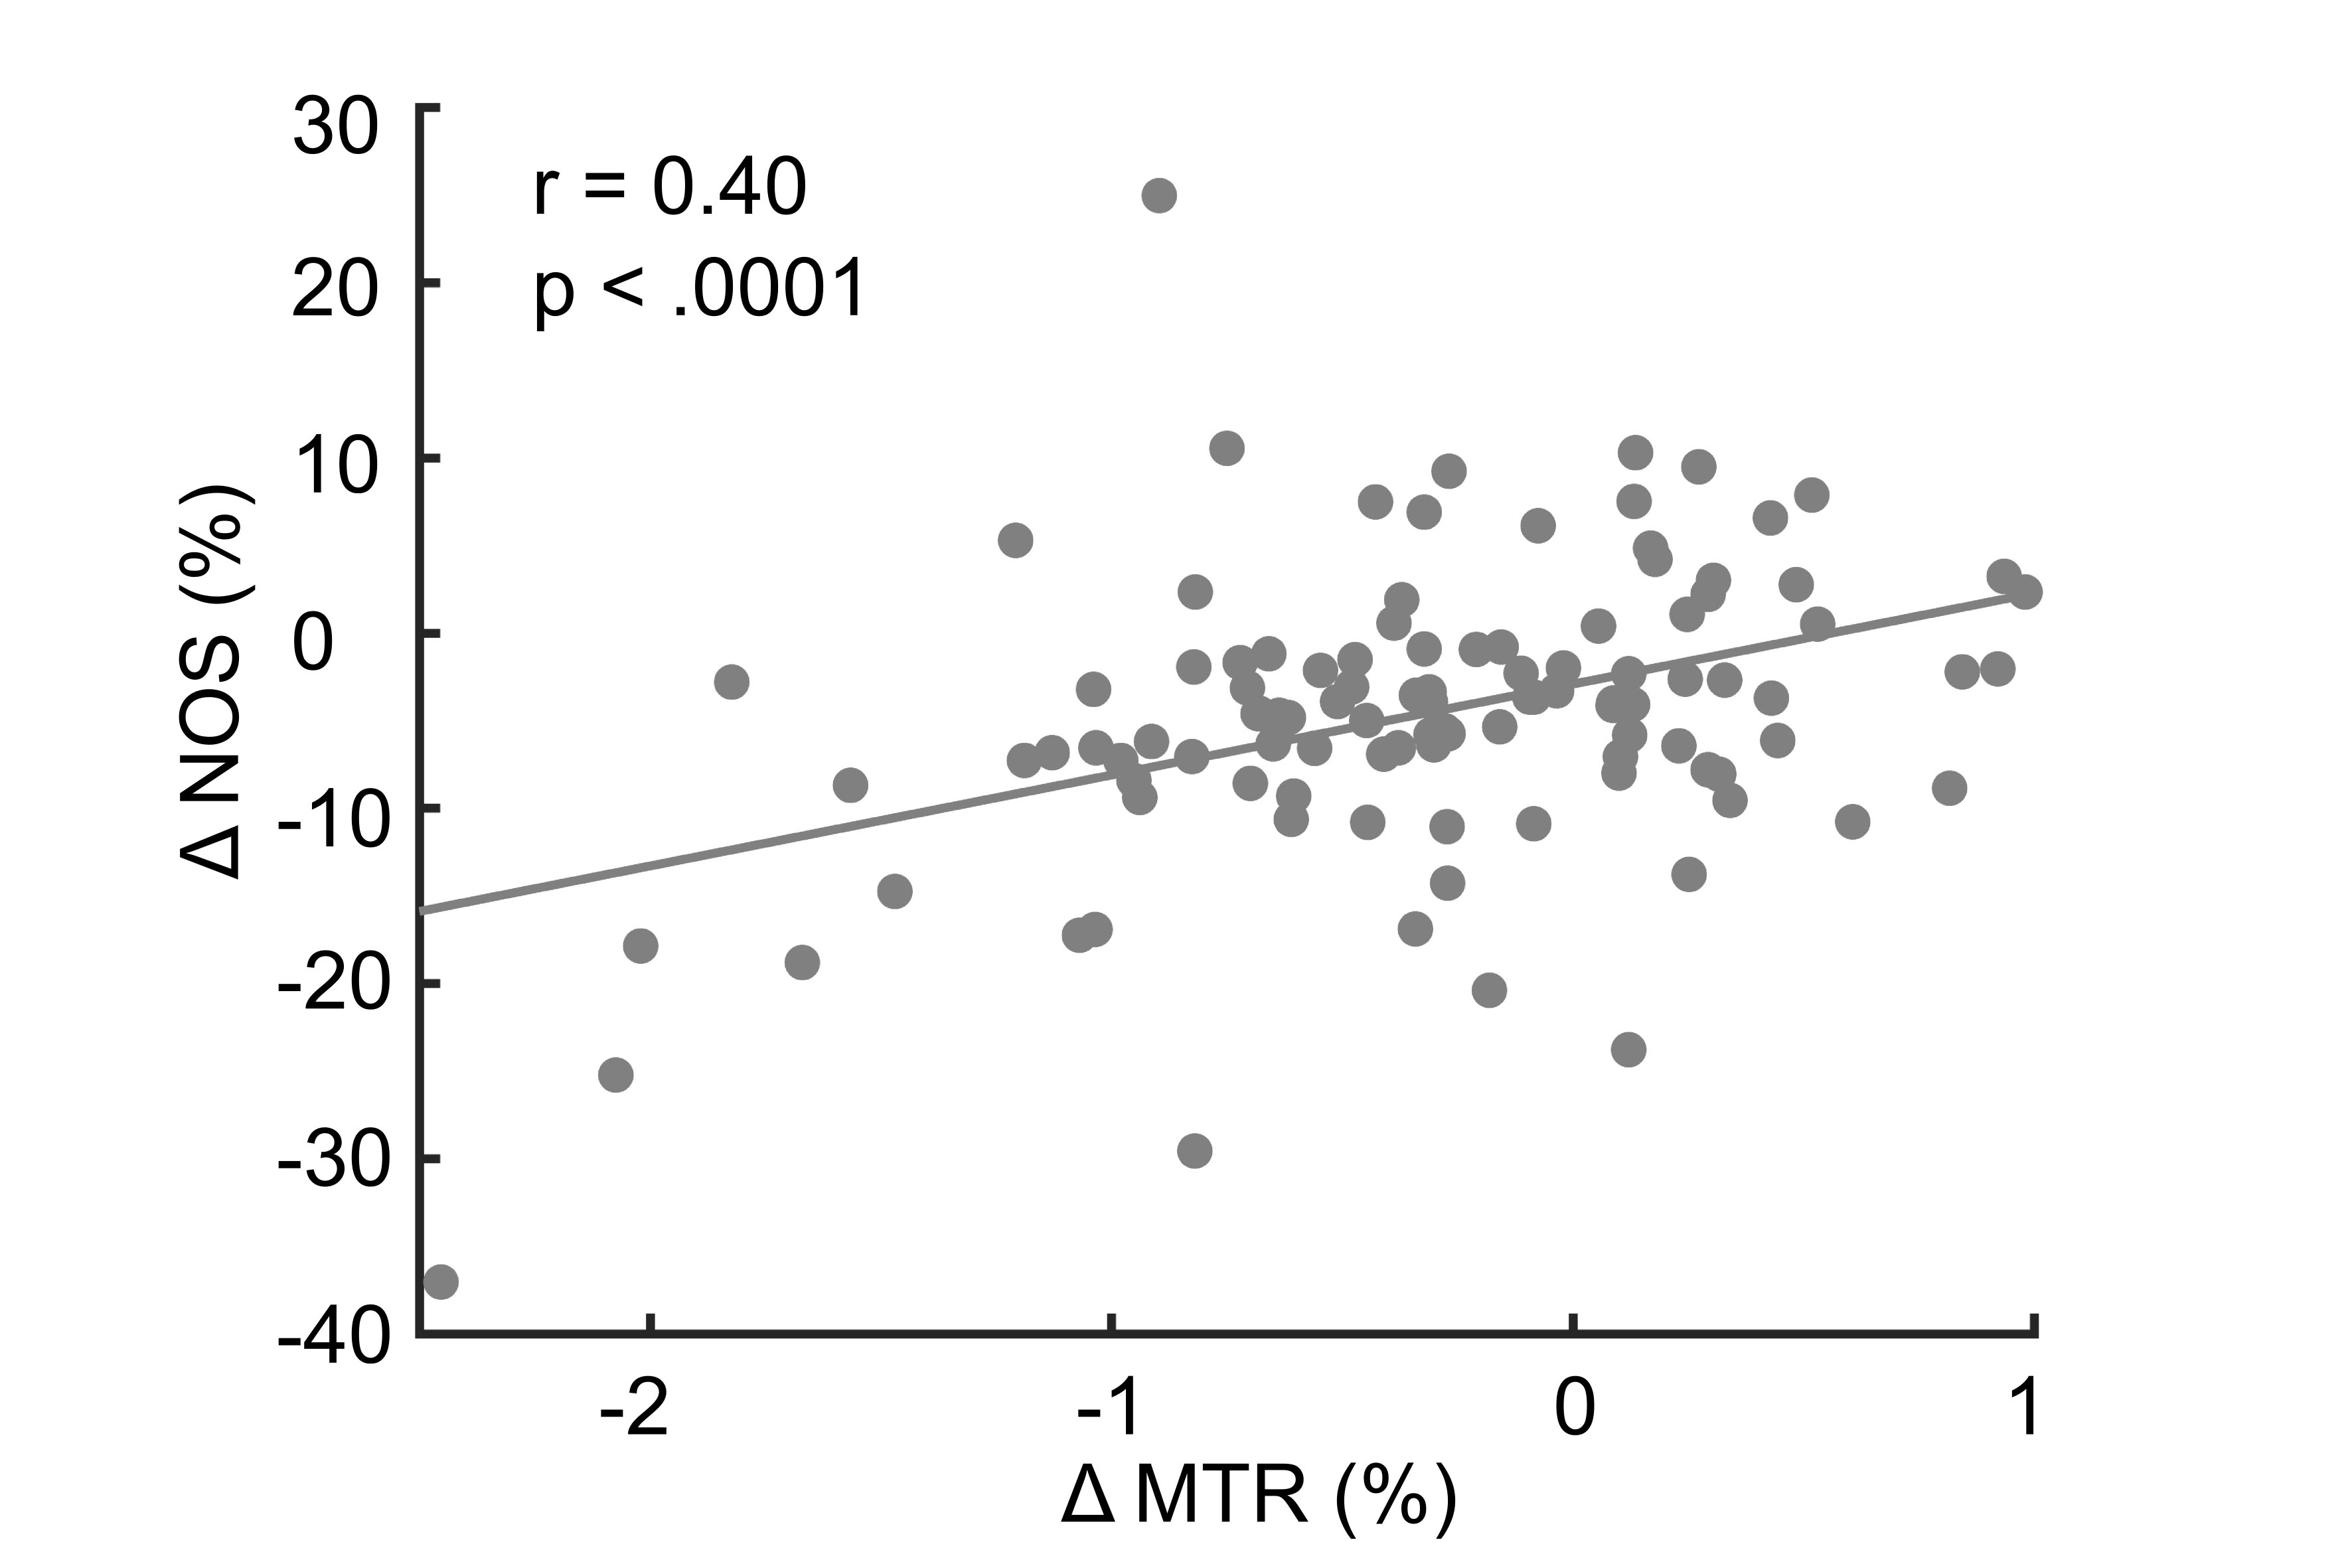
\includegraphics[width=8cm]{images/mtrFig3.jpg}
    \caption{Association between MTR alterations (i.e. $\Delta$ MTR) and connectivity strength changes. $\Delta$ MTR was calculated as the change in group-averaged MTR between schizophrenia patients and controls (i.e., {[}Patient – Control{]}/Control). Changes in cortical connectivity strength are represented by the change in total number of streamline ($\Delta$ NOS) (\rval = 0.40, \pval < 0.0001).}
    \label{mtrFig3}
\end{figure}

\begin{figure}[h]
    \centering
    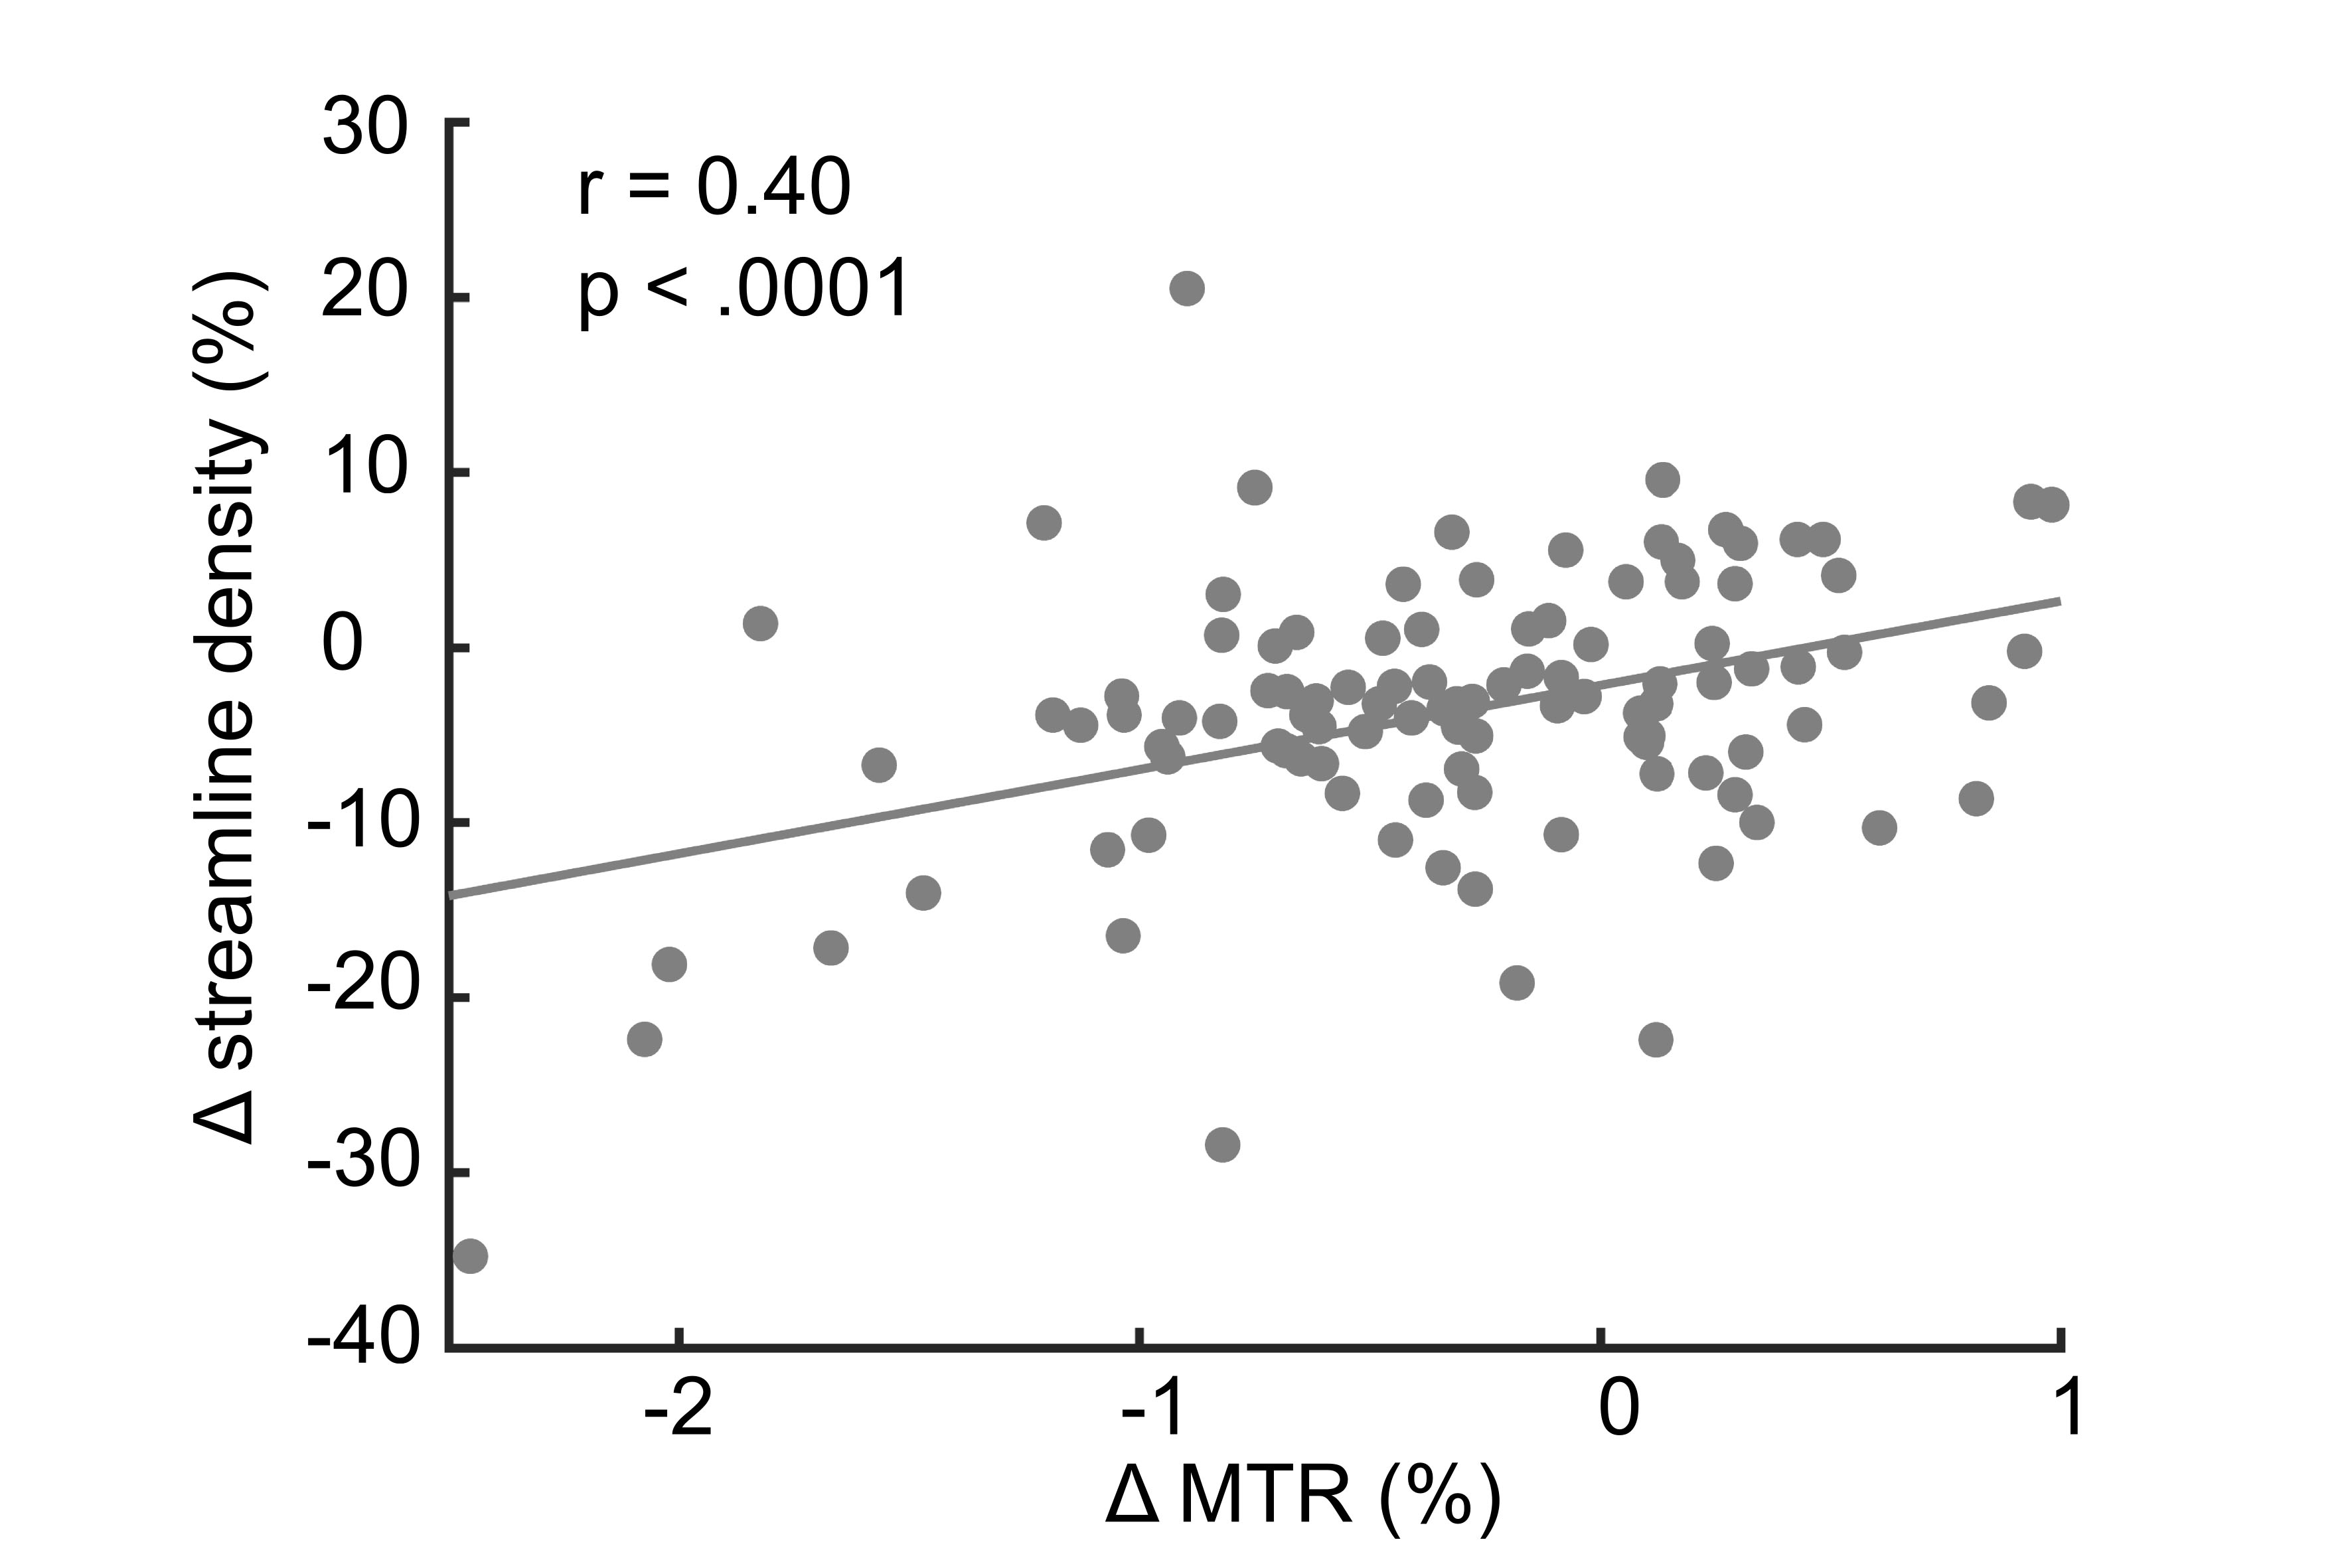
\includegraphics[width=8cm]{images/mtrFig4.jpg}
    \caption{Association between MTR alterations (i.e. $\Delta$ MTR) and connectivity strength changes. $\Delta$ MTR was calculated as the change in group-averaged MTR between schizophrenia patients and controls (i.e., {[}Patient – Control{]}/Control). Changes in cortical connectivity strength are represented by the change in total streamline density ($\Delta$ streamline density) (\rval = 0.40, \pval < 0.0001).}
    \label{mtrFig4}
\end{figure}

Findings persisted when we took changes in cortical thickness and cortical volume into account (NOS: \rval = 0.38, \pval < 0.0001; streamline density: \rval = 0.39, \pval < 0.0001). We alternatively used ranksum values resulting from Wilcoxon Rank Sum test as measurements for between-group differences of MTR and connectivity strength. Regional reductions in MTR consistently showed a significant association with differences in connectivity strength (NOS: \rval = 0.37, \pval = 0.0001; streamline density: \rval = 0.33, \pval = 0.0006). Including changes in cortical thickness and cortical volume as covariates showed similar results (NOS: \rval = 0.34, \pval = 0.0003; streamline density: \rval = 0.31, \pval = 0.0011).


\section*{Discussion}
The present study reveals significant cortical MTR abnormalities in prefrontal cortical areas in schizophrenia, including bilateral rostral middle frontal areas, the right pars orbitalis, and the right frontal pole, suggestive of a prefrontal disruption of macromolecules such as myelin. Second, the cortical pattern of MTR reduction was found to be associated with regional decreases in the level of white matter connectivity in schizophrenia patients relative to controls. These findings provide empirical evidence for microstructural cortical abnormalities of the prefrontal cortex in schizophrenia and suggest that deficits on the microscale are associated with alterations in macroscale structural connectome architecture.

The observed prefrontal MTR abnormalities are compatible with prior cytoarchitectural and myeloarchitectural findings in schizophrenia. Decreased neuronal size of layer III pyramidal neurons has been reported in the prefrontal area (e.g., Brodmann area [BA] 9) in schizophrenia \citep{Pierri2001DecreasedSS,Rajkowska1998NeuronalAG}. Moreover, the density of oligodendroglial cells, which are responsible for forming myelin sheath around axons, has been shown to be reduced in BA 9 and BA 10 in schizophrenia \citep{Hof2003LossAA,Uranova2001ElectronMO,Uranova2004OligodendroglialDI}. The frequency of pathologically myelinated fibers has been reported to be significantly increased in prefrontal area BA 10 in schizophrenia patients \citep{Uranova2011UltrastructuralAO} and gene studies further reported reduced expression of myelin-related and oligodendrocyte-related genes in the prefrontal cortex of patients with schizophrenia \citep{Pierri2001DecreasedSS,Mimmack2002GeneEA,Pongrac2002GeneEP}. As MTR is thought to be reflective of macromolecular structures in the cortex such as myelin and cell membrane \citep{wolff1994magnetization}, MTR reductions observed in the current study may be related to these microstructural disruptions in schizophrenia. Hence, our findings provide additional in vivo evidence for neuropathological abnormalities in the prefrontal cortex in schizophrenia. 

MTR abnormalities in schizophrenia are observed to be correlated with alterations in white matter connectivity in our study. This provides indirect support for a relationship between histological features of cortical microsctructure and macroscale connectivity. Macroscale topological properties of white matter connectivity have been reported to be associated with spine count and density of cortical layer III pyramidal neurons \citep{VANDENHEUVEL2016293} and layer III neuronal size \citep{Heuvel2015BridgingCA} in the healthy human brain. Furthermore, alterations in macroscale white matter connectivity in schizophrenia patients were correlated with changes in spine density of cortical layer III pyramidal neurons \citep{VANDENHEUVEL2016293}. These findings indicate that disruptions in macroscale white matter connectivity may reflect long-range axon abnormalities that accompany cortical microscale connectivity changes. Brain disconnectivity in schizophrenia has been hypothesized previously to be related to myelination disruptions caused by reduced oligodendrocytes \citep{Cassoli2015DisturbedMI}, due to myelin regulate the velocity and synchrony of inter-cortical impulse conduction \citep{Fields2008WhiteMI}. Our findings may provide empirical evidence for this micro-macro association, showing cortical regions with myelination disruptions as revealed by in vivo MTR to be related to the pattern of macroscale disconnectivity in schizophrenia. 

The underlying processes that drive the observed association between MTR abnormalities and white matter connectivity disruptions in schizophrenia remains to be determined. It is known that the streamline number or density measured by diffusion MRI can reflect multiple microscale characteristics, such as axonal number, density, caliber, or myelination \citep{Jones2013WhiteMI}. One hypothesis to explain the MTR-connectivity association could be that reduced white matter connectivity reflects a reduced number or density of axons, which may lead to a decreased intra-cortical myelin content revealed by MTR. Alternatively, pathologically altered intracortical myelination may disrupt neural impulse conduction, and thereby lead to pruning of axons revealed by macroscale connectivity strength. Furthermore, a rich body of literature has reported longitudinal disease effects on both the microscale and macroscale of brain organization \citep{Bullmore1997TheDN,Catani2005TheRA}. The observed association may thus also reflect a more complex bidirectional process of interactions between microstructural abnormality in gray matter and macroscale disconnectivity during the course of disease. 

The putative impact of cortical thinning \citep{Goldman2009WidespreadRO,Haren2011ChangesIC} on our findings was thoroughly examined. We adopted a weighted average measurement for MTR that minimizes the contribution of voxels located in the boundaries of the cortical ribbon. Cortical thickness and volume were regressed out from MTR during statistical analysis. In addition, the validation analysis of the potential cortical thinning effect on MTR between subgroups divided by cortical thickness did not change the results (see Supplementary Information), further indicating that our MTR findings are likely to be independent of cortical thinning effects.

Several other comments have also to be made when interpreting the findings of our study. First, most patients (>85\%, see the Section Subjects) received antipsychotic treatment that might affect the intracortical MTR metric. Examining the relationship between antipsychotic medication dosage and MTR, we found no significant correlations, suggesting that our findings are unlikely driven by antipsychotic medication use. Second, there was a male predominance in the patient group. Post-hoc comparisons revealed MTR reductions between schizophrenia patients and controls in males only, but not in females (see Supplementary Information). This may be due to the small sample size of female patients (\textit{N} = 14) included in our study, or may reflect stronger effects in male as compared to female patients. After randomly excluding female controls to make the gender distribution matched, we consistently found significant MTR reductions in the four reported prefrontal regions (see Supplementary Information), indicating that our findings were likely not driven by a gender effect. Third, the cortical MTR of the four prefrontal areas that showed reductions in schizophrenia only weakly correlated with the WLT retention rate, but did not correlate with other clinical symptoms and cognitive variables. It is probably because of the fluctuating nature of clinical symptoms that change with psychotic episodes and remissions, while MTR findings represent structural deficits that may reflect an underlying neurobiological vulnerability. Finally, given that the included data is part of a long running clinical cohort, the MTR and DWI data included relatively low resolution data acquired on a 1.5 T clinical scanner. Nevertheless, we noticed that MTR data showed acceptable reliability because of high tissue contrasts, high signal to noise ratios, and relatively low within-subject signal variances (see Supplementary Information). Future studies deploying high-field imaging will enhance image quality with higher resolution and higher signal to noise ratios, which may result in less partial volume effects for MTR extraction and better detection of white matter tracts in DWI.

This study shows significant MTR reductions in prefrontal cortex areas in schizo-phrenia patients and a significant association of MTR abnormalities with alterations in white matter connectivity in schizophrenia. Our findings provide in vivo support for cytoarchitectural and myeloarchitectural disruptions of the prefrontal cortex in schizo-phrenia and emphasize a link between microscale neuropathology and disease-related connectome alterations, suggestive of a complex etiology that crosses multiple scales of connectome organization.

\printbibliography[heading=subbibliography]

\end{refsection}

% SI
\newpage
\begin{refsection}
\section*{Supplementary Information}
\subsection*{MTR reliability analysis}
We examined the reliability of MTR signals in three ways, by analyzing tissue contrast, signal to noise ratio (SNR), and individual variance in MTR signals. First, we extracted the mean MTR signal within distinct brain tissues (i.e., gray matter, white matter and CSF) for each subject. As shown in Figure \ref{mtrFigS1}, the mean MTR signals in gray matter (0.5522 $\pm$ 0.0095) were lower than signals in white matter (0.6020 $\pm$ 0.0086), but substantially larger than signals in CSF (0.2384 $\pm$ 0.0451), indicating reliable signal contrast in MTR images.

Second, we calculated the SNR based on MTR signals extracted in the gray matter for each subject. SNR was defined as the ratio of the mean (\textmu) to the standard deviation (\textsigma) of the MTR signal:

\[\mathsf{ SNR = \frac{\mu}{\sigma}} \] 

We found that the SNR ranged from 6.60 to 15.05, with a mean value of 10.26, consistent with an acceptable SNR level according to the Rose criteria, which define scans with SNR $\mathsf{\geq}$ 5 as acceptable \citep{Bushberg2011TheEP}.

Third, we computed within-subject MTR variance for each dataset as follows:

\[ \mathsf{VAR_{within-subject} = \frac{1}{N-1}\sum_{i=1}^{n}(MTR_{i}-\mu)^{2}} \]

where \textit{N} is the number of cortical regions, MTR\textsubscript{i} the mean MTR within region \textit{i}, and $\mathsf{\overline{\mu}}$ the mean MTR among all cortical regions. Likewise, between-group MTR variance was calculated for each cortical region:

\[\mathsf{VAR_{between-group} = \frac{1}{N_{groups}-1} \sum_{i=1}^{N_{groups}} n_{i}(\overline{\mu}_{i} - \overline{\mu})^2}\]

where \textit{N\textsubscript{groups}} is the number of groups (here, \textit{N\textsubscript{groups}} = 2), \textit{n\textsubscript{i}} the number of subjects in the group \textit{i}, $\mathsf{\overline{\mu}_{i}}$ the mean MTR in subjects of the group \textit{i}, and $\mathsf{\overline{\mu}}$ the mean MTR in all subjects. We found that the VAR\textsubscript{within-subject} ranged from 0.0001 to 0.0010 in schizophrenia patients and from 0.0001 to 0.0011 in controls (Figure \ref{mtrFigS2}). VAR\textsubscript{between-group} of the four regions showing significant MTR reductions in patients (i.e., the bilateral rostral middle frontal area, the right pars orbitalis, and the right frontal pole) ranged from 0.0040 to 0.0094, which is 13 to 31 times larger than the average VAR\textsubscript{within-subject}. These findings show that MTR differences between schizophrenia patients and controls are much larger than within-subject MTR measurement variance.

\subsection*{Validation analysis: potential effect of cortical thinning}
We performed a reliability analysis to examine whether cortical thinning effects were not driving the MTR group-effect shown in the main text. To this end, for each region showing a significant between-group MTR difference, we ordered subjects according to cortical thickness and split each group into two subgroups, i.e. schizophrenia patients with above-average thickness (\textit{n} = 38) and with below-average thickness (\textit{n} = 37), as well as controls with above-average thickness (\textit{n} = 45) and with below-average thickness (\textit{n} = 44). Wilcoxon Rank Sum permutation analyses were performed to compare regional MTR measurements between each set of subgroups. We found no MTR differences between patients (or controls) with above-average thickness versus patients (or controls) with below-average thickness (\textit{p}s > 0.1292). Moreover, comparing controls with below-average thickness to patients with above-average thickness again showed MTR reductions in the four prefrontal regions (i.e., bilateral rostral middle frontal area (\pval = 0.0001 and 0.0197), right pars orbitalis (\pval = 0.0264), and right frontal pole (\pval = 0.0022)), indicating that cortical thinning effects are not driving group-effects in MTR.

\subsection*{Gender effects on MTR findings}
We examined the effects of group-gender differences on our MTR findings in two ways, as there was a higher proportion of males in the patient group (e.g., 42 males and 47 females in controls, 62 males and 14 females in patients, \textchi\textsuperscript{2} = 20.80, \pval < 0.0001). First, Wilcoxon Rank Sum permutation analyses, which estimate the difference between medians of the two groups, were performed between cortical MTR of schizophrenia patients and controls in male and female subjects only. This analysis confirmed MTR reductions in the bilateral rostral middle frontal area, the right pars orbitalis, and the right frontal pole between 62 male patients and 42 male controls (\pval = 0.0090, 0.0010, 0.0007, and 0.0078, separately) (Figure \ref{mtrFigS3}). The effects were remained in left rostral middle frontal area (\textit{p} = 0.0222) when comparing the 14 female patients to 48 female controls, but not in other three regions (\pval = 0.1892, 0.1858, and 0.1491, separately), which may be due to either weaker group-effects in female subjects or reduced sample size and power (i.e., testing only 14 female patients). To investigate whether there is a general gender-related MTR difference, the same analysis was also conducted in 42 male controls and 48 female controls. We found no MTR differences in bilateral rostral middle frontal area (\pval = 0.1296 and 0.1196) or right pars orbitalis (\pval = 0.7230), but a trend towards higher MTR values in female controls for the right frontal pole (\pval = 0.0244). These findings suggest that there may be subtle gender-related differences in MTR for some brain regions, but show that our main group-effects in MTR is not driven by group-differences in gender distribution.

Second, we reassessed MTR group-differences using a subgroup of gender-matched controls. We randomly excluded 37 female controls to obtain a gender-matched subgroup (patients: 62 males/14 females; controls: 42 males/10 females, \textchi\textsuperscript{2} = 0.01, \pval = 0.9082) and redid the between-group MTR comparison. The randomization process was repeated for 1000 times and p values for the four significantly different prefrontal regions in our primary analysis (i.e., bilateral rostral middle frontal area, right pars orbitalis, and right frontal pole) were recorded for each randomization. MTR reductions were found in 964 of the 1000 randomizing trials for all those four regions, further supporting that the main group-effects in MTR is not driven by gender effect.

\subsection*{Supplementary References}
\printbibliography[heading=none]

\newpage
\subsection*{Supplementary Figures}
\begin{figure}[H]
\centering
  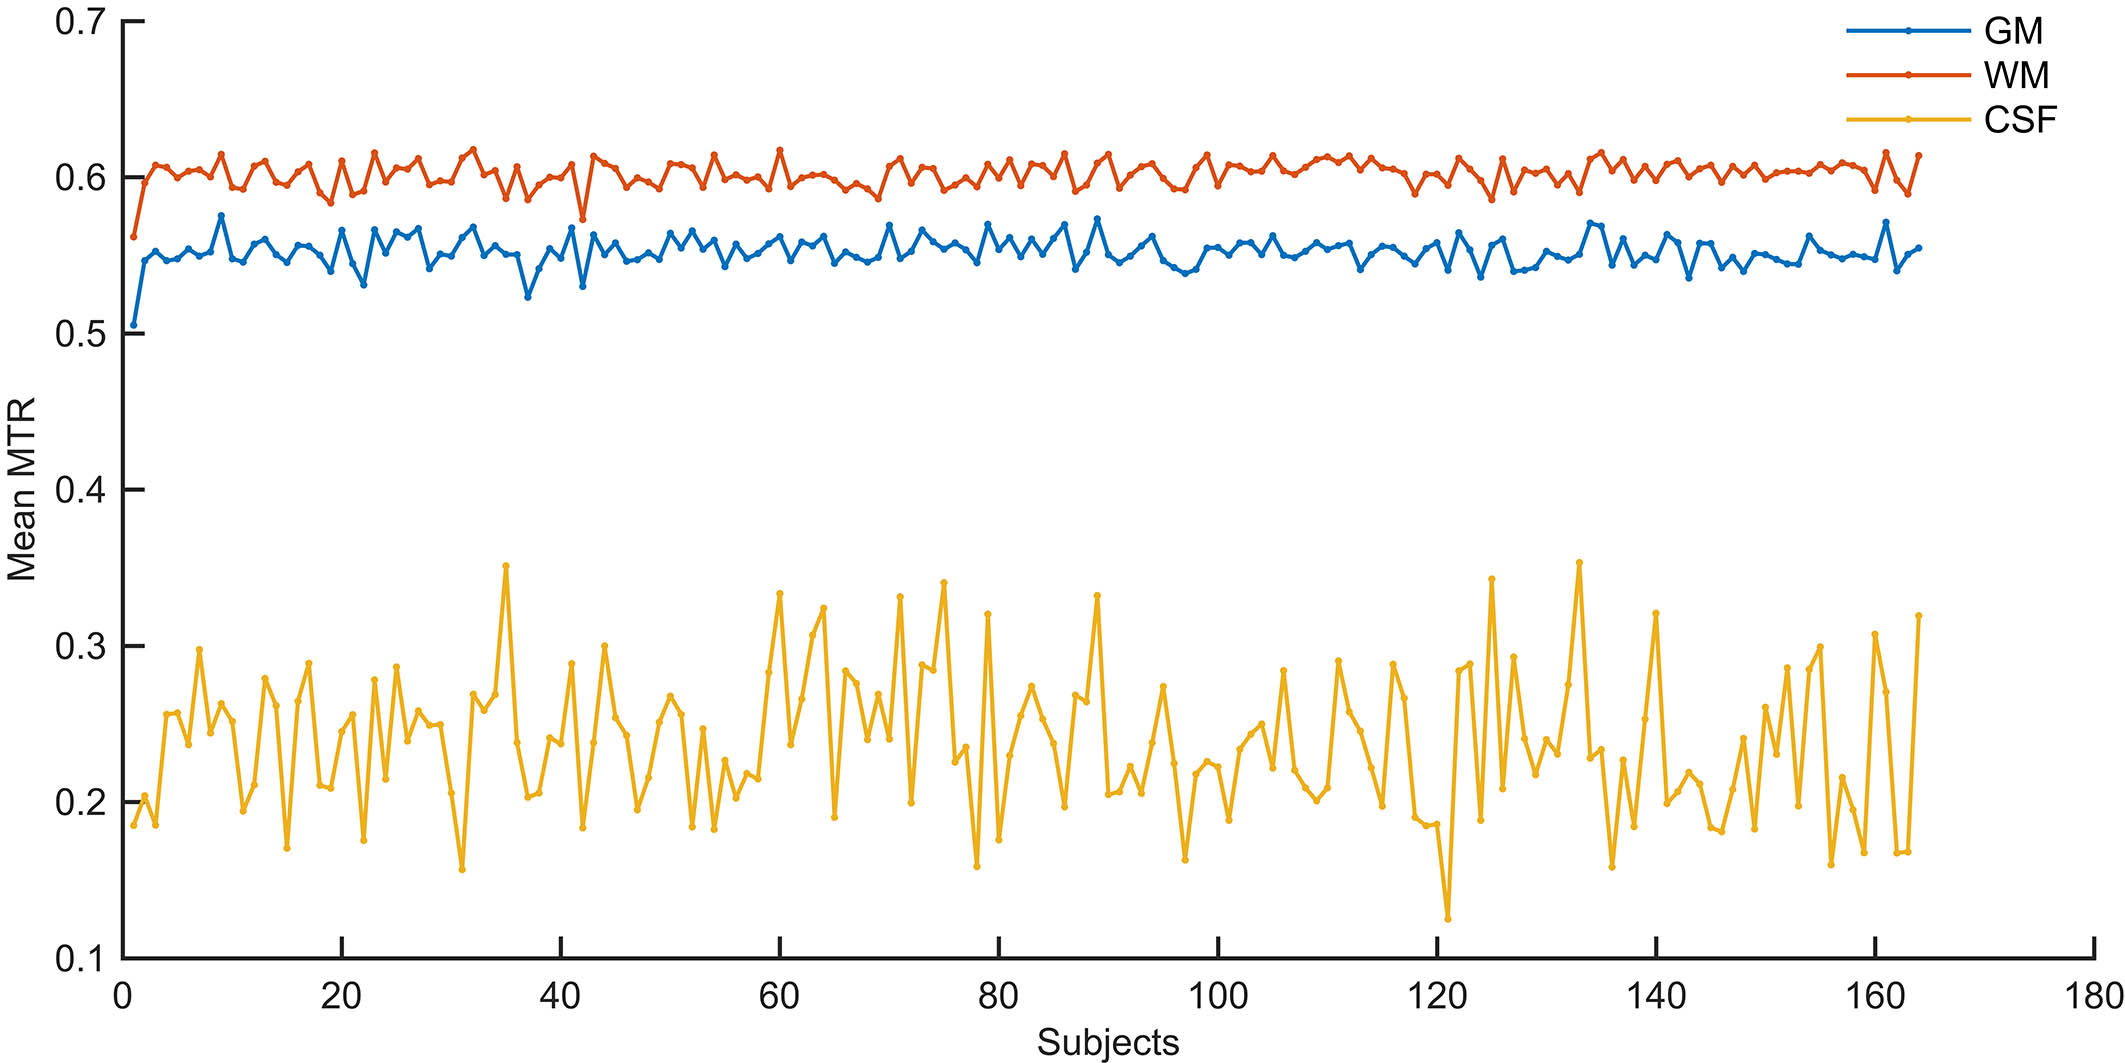
\includegraphics[width=\linewidth]{images/mtrFigS1.jpg}
  \caption{\small Mean MTR signals within gray matter, white matter and CSF for each subject. Blue: gray matter; red: white matter; yellow: CSF.}
  \label{mtrFigS1}
\end{figure}

\begin{figure}[H]
\centering
  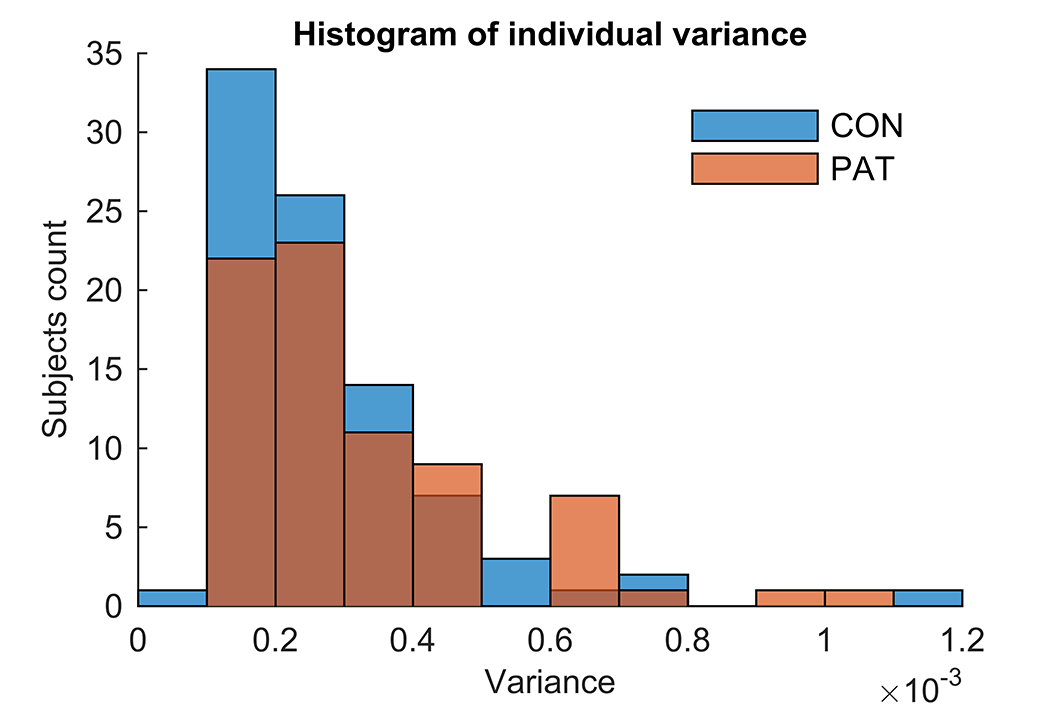
\includegraphics[width=8cm]{images/mtrFigS2.png}
  \caption{\small Histogram of within-subject variances for MTR in each subject. Blue: controls (CON); orange: schizophrenia patients (PAT).}
  \label{mtrFigS2}
\end{figure}

\begin{figure}[H]
\centering
  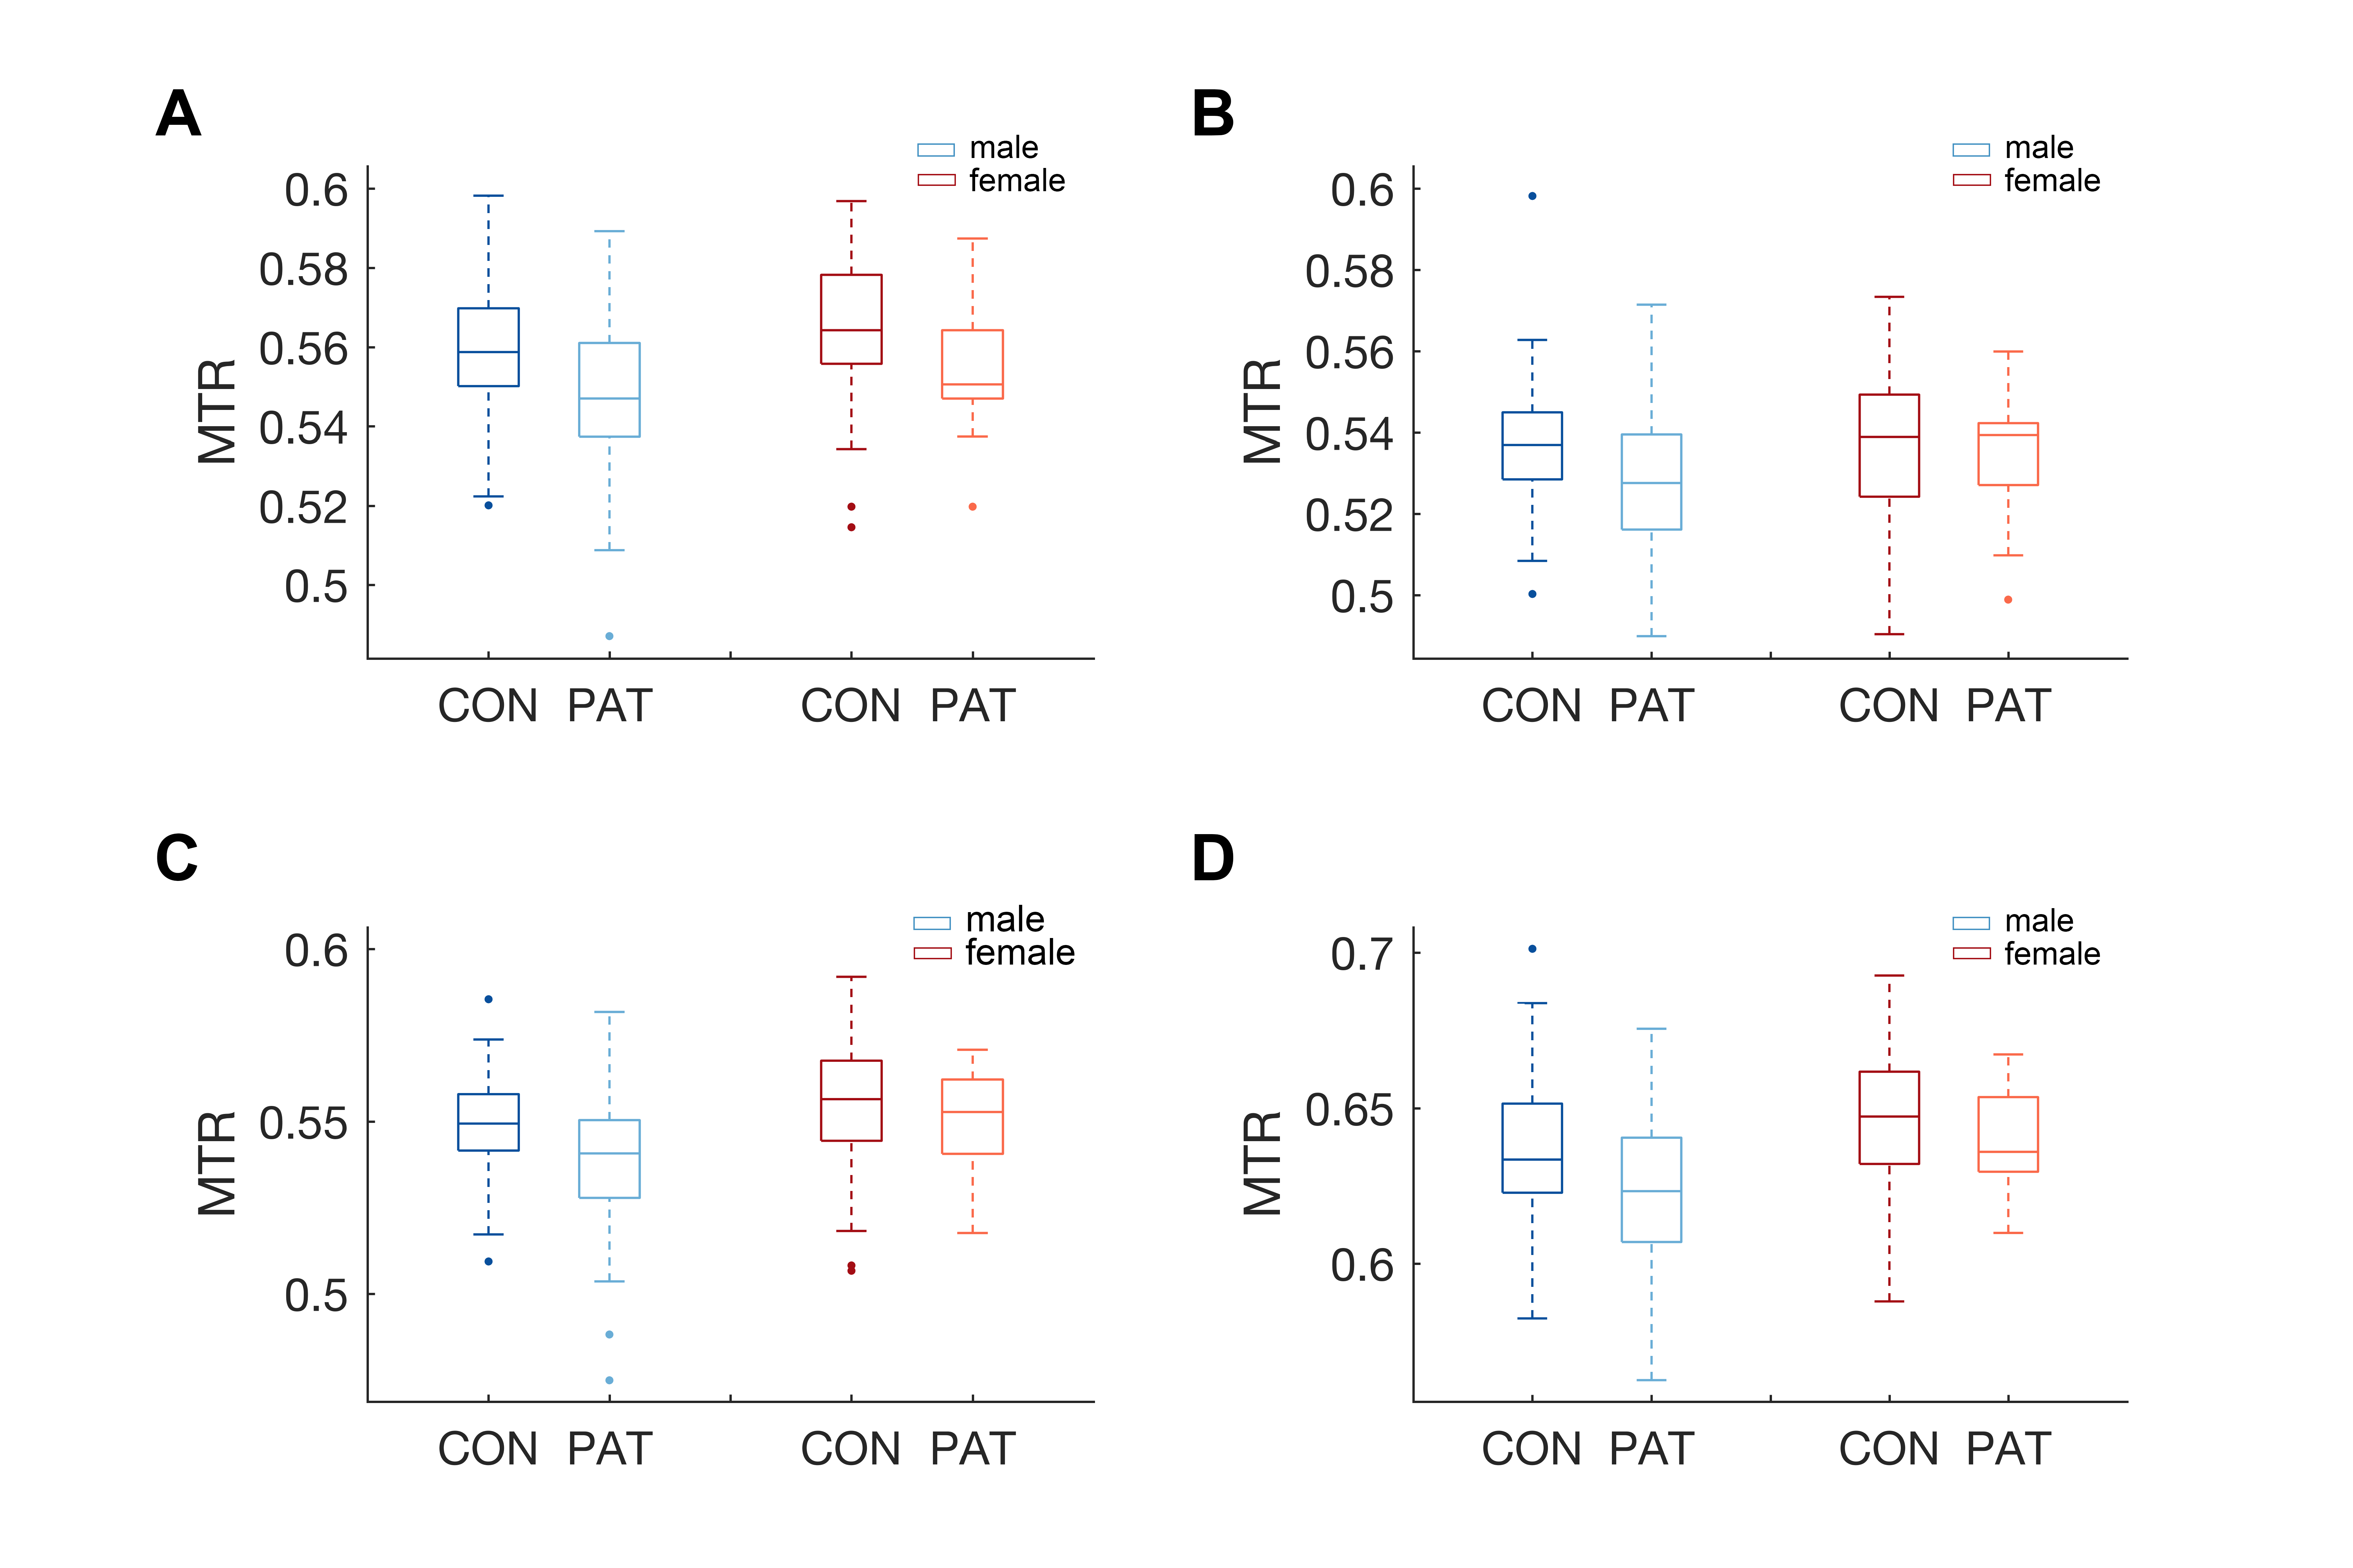
\includegraphics[width=\linewidth]{images/mtrFigS3.png}
  \caption{\small Boxplots of the MTR in the bilateral rostral middle frontal area (left hemisphere: A and right hemisphere: C), right pars orbitalis (B) and the right frontal pole (D). On each boxplot. the central mark on each box is the median, the edges of the box are the 25th and 75th percentiles, the whiskers extend to the most extreme data points considered not to be outliers according to interquartile range (IQR) algorithm, and the outliers are plotted individually. Blue: male, red: female, darker: controls, lighter: patients.}
  \label{mtrFigS3}
\end{figure}



\end{refsection}

